\documentclass[11pt]{article}
\usepackage{graphicx}
\usepackage{tikz}
\usetikzlibrary{shapes.geometric, arrows}
\tikzstyle{arrow} = [thick,->,>=stealth]
\usepackage{pgfplots}
\usepackage{subfig}
\usepackage{float}
\usepackage{amsmath}
\usepackage{boisik}
\usepackage[OT1]{fontenc}
\pagenumbering{roman}
\PassOptionsToPackage{hyphens}{url}\usepackage{hyperref}

%\pagestyle{empty}       % Uncomment if don't want page numbers
\parskip 7.2pt           % sets spacing between paragraphs
%\renewcommand{\baselinestretch}{1.5} % Uncomment for 1.5 spacing between lines
\parindent 0pt		 % sets leading space for paragraphs


\begin{document}
\title{Towards Linking Mammography and Breast Histology Images Using Diffusion Models}
\author{Louai Zaiter$^{1}$\\ loz2@aber.ac.uk }


\date{}
\maketitle
\begin{abstract}
An ever-increasing rate of breast cancer occurrence has led to the development of deep learning techniques to diagnose cancer from medical images. This study introduces a machine learning model to link mammography and breast histology images. We employ a latent diffusion model that uses a variational autoencoder along with a modified UNet model to generate synthetic histology images from input mammograms. We introduce a novel way to train the UNet model that resulted in the synthesis of high resolution histology images. The generated histology images are fed into a deep learning classifier that returns the label of each patch i.e. bening or malignant.
\end{abstract}

\section{Introduction}
 Breast cancer diagnosis is performed in two steps i.e. the mammography screening and the biopsy. In the first step, the radiologist check whether the mammogram is normal or abnormal. If there is an abnormality, the patient might undertake a tissue biopsy which will be evaluated by a pathologist. 

 This study introduces a novel deep learning model to predict how the histology image might look like while having only a mammography as input. We generated our own dataset by combining pairs of mammography and histology images from two publicly available datasets. We propose a lightweight variational autoencoder architecture in order to mammography embeddings and to reconstruct the latent space vector into a histology images. We trained a modified UNet model to find the mapping between the histology embeddings and the mammography embeddings. To evaluate the deep learning model we fed the generated histology images into a trained ResNet50 model in order to predict the label of each image.

 The rest of the paper is divided as follows; section 2 presents the related works, section 3 is for defining the key terms, section 4 is about the dataset used during this study, section 5 introduces the methodology, section 6 presents the results and findings, and the last section is a conclusion 

 \section{Related Work}
 \subsection{Histology synthesis}
 Levine et al. \cite{levine2020synthesis} proposed a deep learning framework that is able to generate synthetic breast histopathology images using generative adversarial networks (GANs) and classify the generated pathology images using a pre-trained deep convolutional neural network (DCNN); the VGG19. In order to preprocess the data extracted from public databases, their study used data augmentation and HSV color normalization. To generate histology images, the progressive GAN is used which consists of a generator and a discriminator where the generator generates fake pathology images which are used to fool the discriminator.
Xue et al. \cite{xue2021selective} proposed a conditional GAN architecture named HistoGAN that has the ability to generate synthetic images and eventually augment the original dataset with realistic histology images. The generator used self attention layers along with residual blocks. Generated fake images goes through a feature extractor network. The extracted features are, then, fed to an image selector and combined with the original dataset. The resulting dataset is augmented and fed to a deep learning classifier ResNet34. 
Butte et al. \cite{butte2022sharp} introduced Sharp-GAN; a generative adversarial network that is sharpness loss regularized. The generator G utilizes a U-Net based pixel2pixel network with a sharpness loss to enhance the contrast of contour pixels of nuclei. The study proposes the generation of a distance map from binary maps to clear separate nuclei. They compared the outcome of their model with another one without sharpness loss and they have found that the Sharp-GAN outperforms other networks. To evaluate the outcome of their proposed GAN, the author has fed the synthetic and real histology images to segmentation models; Seg-Net and U-Net.
 \subsection{Diffusion models}
Saharia et al. \cite{saharia2022palette} introduced an image-to-image translation model that uses a conditional diffusion model. Their unified framework is tested on colorization, inpainting, and JPEG restoration. To evaluate the proposed model, they used sample quality scores including FID, inception score, and classification accuracy using a ResNet50 model. They concluded that their model outperformed GANs. 
Rombach et al. \cite{Rombach_2022_CVPR} proposed a latent diffusion model for high resolution image synthesis. Their strategy consists of decompressing the image formation into sequential application of denoising autoencoders. The introduction of cross-attention layers into their diffusion model enabled powerful and flexible image generation. 
Kim et al. \cite{Kim_2024_WACV} introduced a latent diffusion model that leverages switchable blocks for image-to-image translation in 3D medical images without patch cropping. Their model exhibited successful image synthesis across different source target modality scenarios. Their proposed model allowed one-to-many modality translation.
\section{Key Terms}
 \subsection{Variational Autoencoders}


\begin{figure}[h!]
        \centering
      \begin{tikzpicture}[scale=0.62, transform shape]
         \tikzset{block/.style= {draw, rectangle, align=center,minimum width=2cm,minimum height=1cm},
         rblock/.style={draw, shape=rectangle,rounded corners=1.5em,align=center,minimum width=2cm,minimum height=1cm},
         input/.style={ % requires library shapes.geometric
         draw,
         trapezium,
         trapezium left angle=60,
         trapezium right angle=120,
         minimum width=2cm,
         align=center,
         minimum height=1cm
      },
         }
         
       \node [block, right of= start, xshift=2cm] (pr) {Encoder};
       
       \node [block, right of= pr, xshift=2cm] (extraction) { Embeddings};
       
       \node [block, right  of= extraction, xshift=2cm] (dr) {Decoder};
      
       
      
       \draw [arrow] (pr) -- (extraction);
       \draw [arrow] (extraction) -- (dr);
      
       ;
      \end{tikzpicture}
      \caption{Autoencoder's building blocks}
      \end{figure}
    
    
By reducing the space dimensionality in the hidden layer, the variational autoencoder manages to recreate an input image. The objective of the autoencoder is to minimize the loss between the reconstructed image and the original image.
    
Variational autoencoders \cite{pinheiro2021variational} are composed of an encoder and decoder. The encoder generates feature vectors that are fed into the decoder in order to reconstruct the input image. The loss function that is geneBreastrally used in autoencoders is the mean squared error (MSE) and the task of the network is to minimize the error between the generated and the original image, meaning that a perfect autoencoder is able to reconstruct the same image. 
    
    
    \begin{equation}
        mse(a,p)= \frac{1}{n} \sum_{i=0}^{n} (a_i - p_i)^2
    \end{equation}
 \subsection{Modified UNet}
 UNet models are generally used for segmentation tasks. The modified UNet model is used to generate embeddings given another input embeddings. The UNet model is composed of three building blocks i.e. The encoder used for downsampling, the bottleneck, and the decoder taht is used for upsampling. For the segmentation task the loss function used is the binary cross entropy with logits and for other tasks, the mean squared error or the L1 loss is used. 

 \begin{figure}[h!]
  \centering
\begin{tikzpicture}[scale=0.62, transform shape]
   \tikzset{block/.style= {draw, rectangle, align=center,minimum width=2cm,minimum height=1cm},
   rblock/.style={draw, shape=rectangle,rounded corners=1.5em,align=center,minimum width=2cm,minimum height=1cm},
   input/.style={ % requires library shapes.geometric
   draw,
   trapezium,
   trapezium left angle=60,
   trapezium right angle=120,
   minimum width=2cm,
   align=center,
   minimum height=1cm
},
   }
   
 \node [block, right of= start, xshift=2cm] (pr) {Downsampling};
 
 \node [block, right of= pr, xshift=2cm] (extraction) { Bottleneck};
 
 \node [block, right  of= extraction, xshift=2cm] (dr) {Upsampling};

 

 \draw [arrow] (pr) -- (extraction);
 \draw [arrow] (extraction) -- (dr);

 ;
\end{tikzpicture}
\caption{Modified UNet's building blocks}
\end{figure}

The modified UNet model aims to generate embeddings that could be decoded by the variational autoencoder in order to generate realistic images.

The combination of autoencoders and UNet models can significantly decrease the execution time while dividing the task into two parts.

\subsection{The Nearest Neighbors Algorithm}
We use an unsupervised nearest neighbors algorithm to find the most similar embedding to the input embedding within the database.

\begin{itemize}
  \item Given an input one dimensional vector, we search for the object that has the lowest distance or the highest similarity within the database.
  \item This includes computing the similarity between the input and all the embeddings within the dataset. 
\end{itemize}

The similarity and distance measures used during this study are:
\begin{itemize}
  \item The cosine similarity that has the following equation: 
  \begin{equation}
    cosine\_similarity = \frac{\sum_i^{n}  A_i B_i}{\sqrt{\sum_i^{n}  A_i^2} \sqrt{\sum_i^{n}  B_i^2}}
  \end{equation}
  \item The manhattan distance which is the sum of the absolute value of the difference between each element in the 1D vector.
  \begin{equation}
    manhattan\_distance = \sum_i^{n} |A_i - B_i|
  \end{equation}
  \item The euclidean distance which is the most used measure within similarity search engines and it has the following formula:
  \begin{equation}
    euclidean\_distance = \sqrt{ \sum_i^{n} { (A_i - B_i)^2}}
  \end{equation}
\end{itemize}


\section{Dataset}
For the mammography part, we used the Breast Cancer Digital Repository (BCDR) \cite{BCDR} dataset and it is composed of 727 patient cases including CC and MLO views. The mammography images has a resolution of 3328 by 4084. The images are saved in TIFF format.

For the histology part, we used the breast histopathological image classification dataset (BreaKHis) \cite{spanhol2015dataset} which is composed of 9019 microscopic images of breast tumor tissue collected from 82 patients using several magnification factors. The dataset contains two classes Benign and Malignant having respectively 2480 and 5429 microscopic images. The size of each image is 700x460 pixels.

We selected 441 images from both datasets and we matched them according to their pathology meaning that benign histology images are matched with benign mammography images and the same case for malignant images. 
 \section{Methodology}
\subsection{Image similarity search}

\begin{figure}[h!]
  \centering
  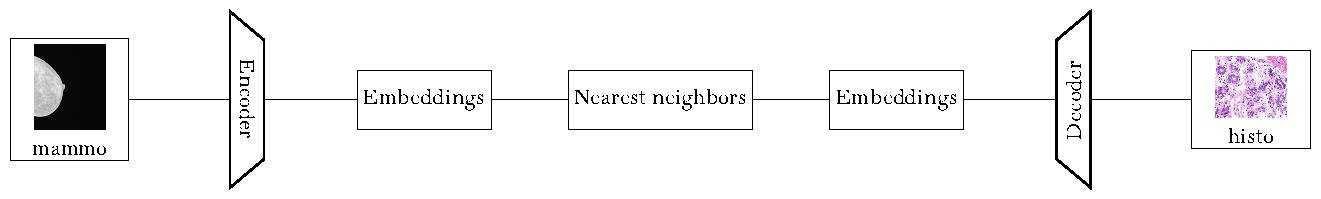
\includegraphics[width=10cm]{similarity_search.pdf}

\caption{The proposed image similarity search framework}
\end{figure}



As shown in Figure 3, we train an autoencoder on the mammography image dataset. Then, we use the trained encoder to generate embeddings for each mammogram and store the results in a database. For a given mammography image, we represent it using an embedding, then, we feed the result into a similarity search engine that uses a k-nearest neighbors algorithm with different similarity measures i.e. the cosine similarity, the Euclidean, and the Manhattan distances. The similarity search engine returns the mammography image that has the highest similarity with the input image. Finally, the algorithm returns the whole slide image associated with the most similar mammogram.

The proposed encoder is composed of five blocks. Each block is made of Convolutional \cite{o2015introduction}, Max pooling \cite{graham2014fractional}, and ReLU \cite{arora2016understanding} layers. The autoencoder is trained during 100 epochs using a mean squared error \cite{willmott2005advantages} (MSE) loss function.

\subsection{Convolutional autoencoders and 1D UNet}
\subsubsection{Single input}

\begin{figure}[h!]
  \centering
  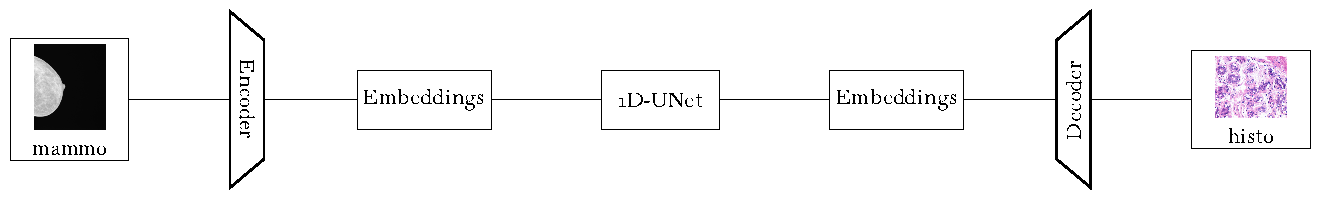
\includegraphics[width=10cm]{Single_input.pdf}

\caption{The proposed image-to-image translation network}
\end{figure}


During this part of the study, we propose implementing an image-to-image translation network that takes as input a mammography image and generates a histology image. The model is composed of two parts i.e. an autoencoder and a one dimensional UNet model. The autoencoder will be trained using mammography and histology images. We use the encoder to generate embeddings from input mammography images, the UNet model will be trained to generate histology feature vectors, and finally, the decoder will be used to synthesize histology images from the histology embeddings.

The proposed UNet model has the following structure:
\begin{itemize}
  \item Down-sampling consists of five blocks each one contains a one dimensional convolutional (Conv1d) layer, a batch normalization layer, and a ReLU activation function
  \item Up-sampling has five blocks each one consists of an Upsample layer, a Conv1D layer, a batch normalization layer, and a ReLU activation function. 
\end{itemize}

In Down-sampling we add a max pooling layer before each block to reduce the dimensions of the resulting tensor. 

As a loss function, we used the MSE in both the autoencoder and the one dimensional UNet model. 

The two proposed autoencoders are trained during 4000 epochs with an Adam optimizer and 1e-4 learning rate. On the other hand, the UNet model took 10000 epochs to converge to the optimal solution. 

\subsubsection{Dual input}
\begin{figure}[h!]
  \centering
  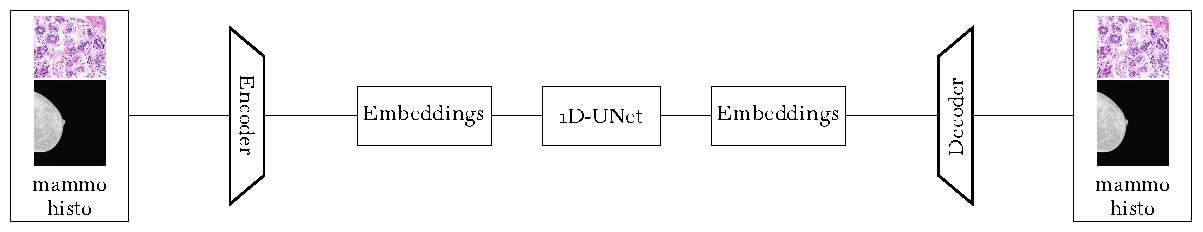
\includegraphics[width=10cm]{dual_input.pdf}

\caption{The proposed dual input image-to-image translation network}
\end{figure}


The dual input image-to-image translation network uses a dual input autoencoder and a 1D UNet model in order to generate pairs of mammography and breast histology images. 

We train two dual input autoencoders i.e. one to generate histology-mammography embeddings and the second is to generate mammography-histology embeddings. Then, we use those two models to train a 1D UNet model the same way as in the previous section.

The dual input autoencoder has the following structure:
\begin{itemize}
  \item The encoder takes as input two images, encode them separately, concatenate the results, and generate a feature vector.
  \item The decoder takes as input a feature vector, and outputs two images. 
\end{itemize}

The dual input encoder is made of two parallel blocks each one uses convolutional, batch normalization, and max-pooling layers. We fuse the features generated by those two blocks, and we apply a dense layer in order to generate a feature vector.

The dual input autoencoders are trained for 4000 epochs and the one dimensional UNet model is trainer for 10000 epochs. In both cases, we use the MSE loss function.
 

\subsection{Diffusion models}
\begin{figure}[h!]
        \centering
        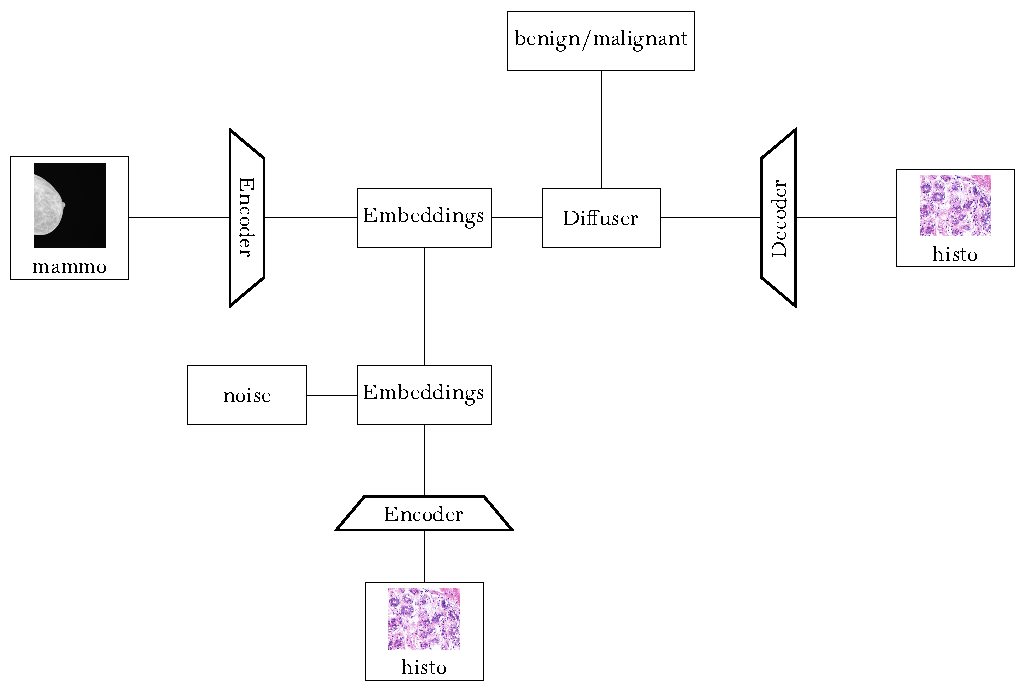
\includegraphics[width=10cm]{diagram_2.pdf}
    
      \caption{The proposed diffusion model architecture during the training phase}
\end{figure}

 The proposed diffusion model is composed of two parts; the variational autoencoder and the modified UNet model. 

 The variational autoencoder has an encoder and a decoder. The encoder has five convolutional blocks and the decoder has five deconvolution blocks. The number of output channels for each block of the autoencoder are 32, 64, 128, 256, and 512. The encoder results in an embedding with 64 channels that will be fed into the modified UNet model. The UNet model manages to find the mapping between the mammography and the histology images and thus enables the generation of synthetic histology images.

 The modified UNet model has a lightweight architecture with two DownSampling blocks and two UpSampling blocks each one having 128 and 256 output channels. 

 During the training phase, we feed the mammography and histology images into the appropriate encoders to generate latent embeddings. Then, we inject noise into the histology embeddings before adding it to the mammography embeddings. The resulting latent space vector is fed into the diffuser model along with the label of each image. Finally, we use the histology decoder to generate synthetic images from the generated embeddings.

 \begin{figure}[h!]
        \centering
        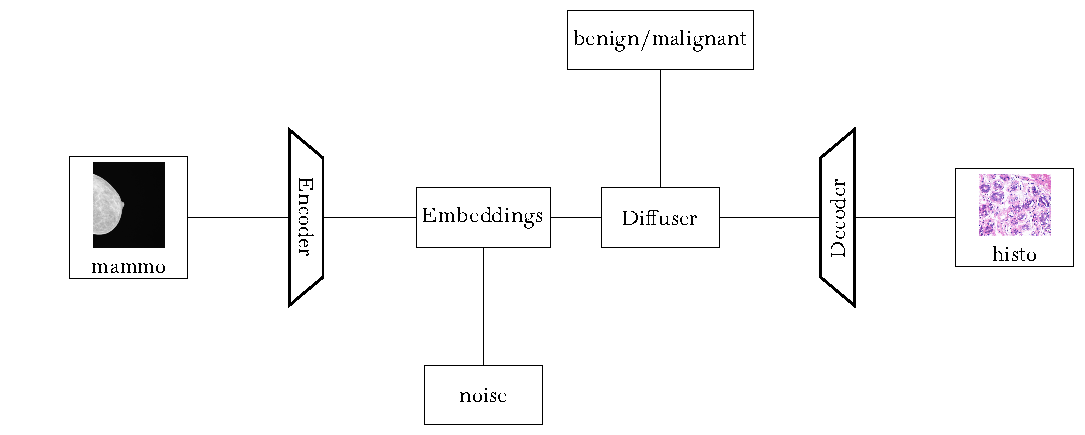
\includegraphics[width=10cm]{test_diagram.pdf}
    
      \caption{The proposed diffusion model architecture during the testing phase}
\end{figure}

During the testing phase, we inject noise into the mammography embeddings, and we feed the result into the modified UNet model as shown in the figure above. To generate synthetic histology images, we gradually denoise the generated latent embeddings. 
\section{Results and Findings}
\subsection{Image Similarity Search Results}


We record the results in Table 1 by comparing the label of the retrieved images with the label of the input image, and we set the number of neighbors in the KNN algorithm to 3.

\begin{table}[h!]
    \caption{ The recorded metrics using different similarity measures }
  \centering
  \scalebox{0.7}{
    \begin{tabular}{|c || c|| c||c|}
      \hline
      Model & precision & recall & accuracy\\ [0.5ex]
      \hline\hline
      Cosine similarity & 84\% & 77\% & 76\% \\
      Manhattan distance & 84\% & 77\% & 77\% \\
      Euclidean distance & 79\% & 63\% & 63\% \\
      \hline
    \end{tabular}}
  
  \label{table:1}
\end{table}

For instance, the algorithm that uses a cosine similarity measure manages to retrieve the correct item with a precision of 84\% and an overall accuracy of 76\%. 

Figure 8 shows the confusion matrices of the best-performing models. The first figure shows that the model has a true positive value of 34 and a true negative value of 63. This confirms the result found in Table 8, indeed, the model has high precision in retrieving the correct image. 

\begin{figure}[!h]
  \centering
  \subfloat[]{\begin{pmatrix}
      34 & 30\\
      0 & 63
  \end{pmatrix}}
  \subfloat[]{  \begin{pmatrix}
      35 & 29\\
      0 & 63
  \end{pmatrix}}
  \quad  
  \caption{The confusion matrices of the models that use a cosine similarity and a Manhattan distance }
\end{figure}
\subsection{Single Input Image-to-Image Translation Network Results}

We evaluate the network by training a ResNet50 classifier to predict the class of the generated histology image. 
\begin{figure}[htp]
\centering
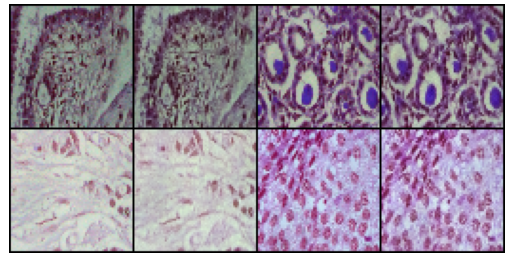
\includegraphics[width=5cm]{test-sample-histo-3.png}

\caption{The generated histology images and their ground truth}
\end{figure}

The ResNet50 with two output neurons is trained for 100 epochs with a cross entropy loss function. In the application phase, we use the mammography encoder to generate embeddings, the one-dimensional UNet model to find the histology feature vector that are fed into the histology decoder. We input the resulting images into a trained ResNet50 that will predict whether the image is benign or malignant. 

Figure 10 shows the generated images using the proposed image-to-image translation network along with their ground truth and Figure 22 is the confusion matrix of the ResNet50 model. The false negative rate is high meaning that 47 malignant histology images are classified as benign. 

\begin{figure}[!h]
  \centering
  \begin{pmatrix}
    73 & 12\\
    47 & 9
    \end{pmatrix}
  \caption{The confusion matrix of the proposed model evaluated using a ResNet 50}
\end{figure}
\subsection{Diffusion model results}

\begin{figure}[htp]
  \centering
  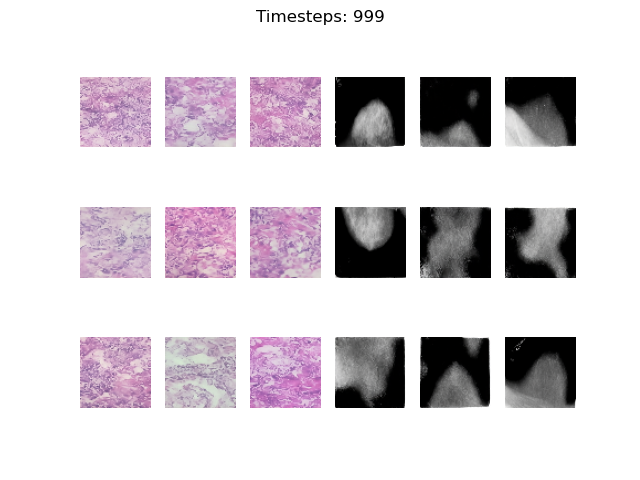
\includegraphics[width=6cm]{sample_1.png}
  
  \caption{The generated histology images and their associated noisy mammography images}
  \end{figure}

Figure 11 shows the generated histology images by the diffusion model along with their associated noisy mammography images. We denoise the histology image during 1000 time steps.

We use a pretrained ResNet50 model to evaluate the generated histology image as in the previous section. 

Figure 12 shows the confusion matrix of the diffusion model evaluated using the testing set of the BCDR dataset. For instance, there are 551 benign images generated by the diffusion model that are correctly classified by the ResNet50 and 1133 malignant images that are misclassified as benign. There are 1045 malignant images that are correctly classified and 433 benign images that are classified as malignant. To conclude, the true negative rate is considerably low compared to the true positive rate.


\begin{figure}[!h]
  \centering
  \begin{pmatrix}
    551 & 433\\
    1133 & 1045
    \end{pmatrix}
  \caption{The confusion matrix of the diffusion model evaluated using a ResNet50}
\end{figure}

 \section{Conclusion}
This study introduced a novel latent diffusion model architecture that uses a combination of variational autoencoders and Unet models. We compared the performance of our proposed network with an image similarity engine and a combination of convolutional autoencoders and one-dimensional Unet model. 
We conclude that the use of diffusion models to link mammography and breast histology images yield the best performance in high resolution image synthesis. 

In further studies, we proposed comparing latent diffusion models with cycle-in-cycle GANs and conditional GANs.
\bibliographystyle{abbrv}
\bibliography{ref}
\end{document}